%=======================02-713 LaTeX template, following the 15-210 template==================
%
% You don't need to this template
%
\documentclass[11pt]{article}
\usepackage{amsmath,amssymb,amsthm}
\usepackage{graphicx}
\usepackage[margin=1in]{geometry}
\usepackage{fancyhdr}
\setlength{\parindent}{0pt}
\setlength{\parskip}{5pt plus 1pt}
\setlength{\headheight}{13.6pt}
\newcommand\question[2]{\vspace{.25in}\hrule\textbf{#1: #2}\vspace{.5em}\hrule\vspace{.10in}}
\renewcommand\part[1]{\vspace{.10in}\textbf{(#1)}}
\newcommand\algorithm{\vspace{.10in}\textbf{Algorithm: }}
\newcommand\correctness{\vspace{.10in}\textbf{Correctness: }}
\newcommand\runtime{\vspace{.10in}\textbf{Running time: }}
\newcommand\tab[1][1cm]{\hspace*{#1}}
\pagestyle{fancyplain}
\lhead{\textbf{\NAME\ (\ANDREWID)}}
\chead{\textbf{HW\HWNUM}}
\rhead{02-713, \today}
\begin{document}\raggedright
%Section A==============Change the values below to match your information==================
\newcommand\NAME{Kadir Emre Oto}  % your name
\newcommand\ANDREWID{150140032}     % your andrew id
\newcommand\HWNUM{1}              % the homework number
%Section B==============Put your answers to the questions below here=======================

% no need to restate the problem --- the graders know which problem is which,
% but replacing "The First Problem" with a short phrase will help you remember
% which problem this is when you read over your homeworks to study.

\question{1}{The first Problem} 

\begin{figure}[h]
	\centering
	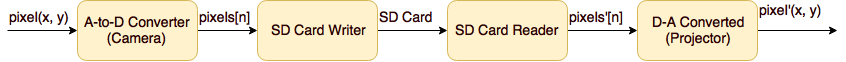
\includegraphics[width=0.7\linewidth]{figure1}
	\caption{Block diagram for a system composed of a digital camera and a projector}
	\label{fig:figure1}
\end{figure}

\question{2}{The second problem}

Roland Priemer defines signal briefly: "A signal is a function that conveys information about the behavior of a system or attributes of some phenomenon" \cite{isp}

\tab \textbf{Figure 1: } A heartbeat record is a signal because it conveys the heartbeat information.

\tab \textbf{Figure 2: } A voice record is also a signal because voice can be represented numerically and transfered between systems.

\tab \textbf{Figure 3: } An image is also a signal because image can be represented as 2 by 2 matrix and conveyed easily. 

\question{3}{The third problem}

\begin{center}
	$ z^4 = j $ \\
	$ z = r \cdot e^{j \cdot Q} = cos(Q) + j \cdot sin(Q)$, where $ Q = \dfrac{\pi}{2}  $ \\
	$ z^4 = e^{j \cdot \left( \frac{\pi}{2} + 2 \cdot \pi \cdot k  \right)} $ \\
	$ z_i = e^{j \cdot \pi \cdot \left( \frac{1 + 4 \cdot k}{8}  \right)} $, where $k = \{0, 1, 2, 3\}$ 
\end{center}
\begin{eqnarray*}
	z_1 &=& e^{j \cdot \frac{\pi}{8}}, \text{where k = 0} \\ 
	z_2 &=& e^{j \cdot \frac{5 \cdot \pi}{8}} , \text{where k = 1}  \\
	z_3 &=& e^{j \cdot \frac{9 \cdot \pi}{8}} , \text{where k = 2} \\
	z_4 &=& e^{j \cdot \frac{13 \cdot \pi}{8}} , \text{where k = 3} \\
\end{eqnarray*}

\question{4}{The fourth problem}
\tab \textbf{Taylor's Formulas:}
	\begin{eqnarray*}
		e^{x} &=& \sum^{\infty}_{n=0} \frac{x^n}{n!} = 1 + x + \frac{x^2}{2!} + \frac{x^3}{3!} + \cdots \\
		\sin x &=& \sum^{\infty}_{n=0} \frac{(-1)^n}{(2n+1)!} x^{2n+1} =  x - \frac{x^3}{3!} + \frac{x^5}{5!} - \cdots \\
		\cos x &=& \sum^{\infty}_{n=0} \frac{(-1)^n}{(2n)!} x^{2n}=  1 - \frac{x^2}{2!} + \frac{x^4}{4!} - \cdots
	\end{eqnarray*}

\tab We can express the equation, $e^{j \theta}$, in terms of the Taylor's Formulas:
	
	\begin{eqnarray*}
		e^{j \theta} &=& 1 + (j \theta) + \frac{(j \theta)^2}{2!} + \frac{(j \theta)^3}{3!} + \frac{(j \theta)^4}{4!} + \cdots \\
		e^{j \theta} &=& 1 + (j \theta) + \frac{-\theta^2}{2!} + \frac{-j \theta^3}{3!} + \frac{ \theta^4}{4!} + \cdots \\
		e^{j \theta} &=& (1 - \frac{\theta^2}{2!} + \frac{ \theta^4}{4!} - \cdots) + j (\theta -\frac{ \theta^3}{3!} +\frac{ \theta^5}{5!} - \cdots) \\
		e^{j \theta} &=& cos(\theta) + j sin(\theta) \\
	\end{eqnarray*}
	
\question{5}{The fifth problem}

\part{a} A function can be called as \textbf{odd} if and only if it satisfies $f(-x) = -f(x)$ These functions are typically symmetric with respect to the origin. 
\begin{center}
	Ex: $ f(x) = x^3 $
\end{center}

\part{b} A function can be called as \textbf{even} if and only if it satisfies $f(-x) = f(x)$ These functions are typically symmetric with respect to y-axis. 

\begin{center}
	Ex: $ f(x) = x^4 $
\end{center}

\part{c} \\
\tab \textbf{a.} $sin(\theta) \rightarrow cos(\theta - \pi / 2) $\\
\tab \textbf{b.} $cos(\theta + 2 \pi k ) \rightarrow cos(\theta) $, when k is an integer \\
\tab \textbf{c.} $cos(-\theta) \rightarrow cos(\theta) $ \\
\tab \textbf{d.} $sin(-\theta) \rightarrow -sin(\theta) $ \\
\tab \textbf{e.} $sin(\pi k) \rightarrow 0$, when k is an integer \\
\tab \textbf{f.} $cos(2 \pi k) \rightarrow 1$, when k is an integer \\
\tab \textbf{g.} $cos \left[ 2\pi \left(k + 1 / 2\right) \right]  \rightarrow -1$, when k is an integer \\

\part{d} \\
\tab \textbf{i.}
	\begin{eqnarray*}
		e^{j\theta} &=& cos(x) + j sin(x), (Euler's Formula) \\
		e^{-j\theta} &=& cos(x) - j sin(x) \\
		e^{j\theta} \cdot e^{-j\theta} &=& cos^2(x) + sin^2(x) \\
		e^0 = 1 &=& cos^2(x) + sin^2(x) \\
	\end{eqnarray*}

\tab \textbf{ii.} 
	\begin{eqnarray*}
		cos(2\theta) &=& Re\left\{ e^{j 2 \theta} \right\} \\
		cos(2\theta) &=& Re\left\{ (e^{j \theta}) ^ 2 \right\} \\
		cos(2\theta) &=& Re\left\{ (cos(\theta) + j sin(\theta)) ^2 \right\} \\
		cos(2\theta) &=& Re\left\{ cos^2(\theta) + 2 j sin(\theta) cos(\theta) - sin^2(\theta) \right\} \\
		cos(2\theta) &=& cos^2(\theta) - sin^2(\theta) \\
	\end{eqnarray*}

\tab \textbf{iii.}
	\begin{eqnarray*}
		sin(2\theta) &=& Im\left\{ e^{j 2 \theta} \right\} \\
		sin(2\theta) &=& Im\left\{ (e^{j \theta}) ^ 2 \right\} \\
		sin(2\theta) &=& Im\left\{ (cos(\theta) + j sin(\theta)) ^2 \right\} \\
		sin(2\theta) &=& Im\left\{ cos^2(\theta) + 2 j sin(\theta) cos(\theta) - sin^2(\theta) \right\} \\
		sin(2\theta) &=& 2sin(\theta)cos(\theta) \\
	\end{eqnarray*}

\question{6}{The sixth problem}
\begin{eqnarray*} \\ 
	\sum_{k=1}^{N} A_k cos(\omega_0 t + \varPhi_k) &=&  A cos(\omega_0 t + \varPhi) \\
	\sum_{k=1}^{N} A_k e^{j \varPhi_k } &=&   A e^{j \varPhi } \text{(The essense of the phasor addition rule)}\  \cite{signalbook} \\
	A cos(\omega_0 t + \varPhi) &=& Re \left\{ A e^{j (\omega_0 t + \varPhi)}  \right\} =  Re \left\{ A e^{j \varPhi} e^{j \omega_0 t}  \right\} \\
	 Re \left\{ \sum_{k=1}^{N} X_k  \right\} &=& \sum_{k=1}^{N} Re \left\{ X_k \right\} \\
	 \sum_{k=1}^{N} A_k cos(\omega_0 t + \varPhi_k) &=& \sum_{k=1}^{N} Re \left\{ A_k e^{j (\omega_0 t + \varPhi_k)} \right\} \\
	&=& Re \left\{ \left( \sum_{k=1}^{N} A_k e^{j \varPhi_k } \right) e^{j\omega_0 t}  \right\} \\
	&=& Re \left\{ \left( A e^{j\varPhi} \right) e^{j\omega_0 t}  \right\} \\
	&=& Re \left\{ A e^{j (\omega_0 t + \varPhi)}  \right\{ \\
	&=& A cos(\omega_0 t + \varPhi) \\
\end{eqnarray*}

\question{7}{The seventh problem}

\question{8}{The eighth problem}

\question{9}{The ninth problem}

\question{10}{The tenth problem}

\question{11}{The eleventh problem}

\question{12}{The twelfth problem}

\question{13}{The thirteenth problem}

\begin{thebibliography}{1}
	\bibitem{isp} 
	Roland Priemer
	\textit{Introductory Signal Processing}. (English) 
	[\textit{World Scientific. p.1}]. ISBN 9971509199, 2013.
	
	\bibitem{signalbook} 
	James H. McClellan., Ronald W. Schafer, Mark A. Yoder
	\textit{Signal Processing First}. (English) 
	[\textit{Phasor Addition Rule 2-6.2}]. ISBN 0-13-120265-0, 2003.
\end{thebibliography}

\end{document}
